% Compile twice with: pdflatex r2_reviewreport.tex
% Keep ssnreview.cls, ssn-logo.png and the figures/ folder in the same folder.
%
% BEFORE SUBMISSION (items shown in red in the PDF):
%   1. Chapter 2 (First Review - Queries and Answers) must be filled in from the
%      Review I minutes. It is intentionally left as placeholders.
%
% NOTE: ssnreview.cls does not load amsmath, so \text, \operatorname, align etc.
% are unavailable. Use \mathrm{} in formulas.
\documentclass{ssnreview}

\projecttitle{Assessment of Alzheimer's Disease Progression Using
Comorbidity-Aware Meta-Bayesian Framework with Resting-State fMRI}
\reviewnumber{REVIEW REPORT -- II}
\students{%
  Harishkanna R (3122235001302)\\
  Dhananchezhiyan M (3122235001041)\\
  Nagindhar Sachein R L (3122235001702)}
\supervisor{Dr.~N. Ahana Priyanka\\Assistant Professor}
\department{Department of Computer Science and Engineering}
\institution{Sri Sivasubramaniya Nadar College of Engineering}
\academicyear{2026--2027}
\collegelogo{ssn-logo.png}

\setlength{\emergencystretch}{3em}

\begin{document}
\makereviewtitle
\reviewfrontmatter

\begin{reviewabstract}
Alzheimer's disease (AD) progresses through intermediate stages that are difficult
to separate using clinical assessment alone, and resting-state functional MRI
(rs-fMRI) offers a non-invasive window onto the functional disruption that precedes
structural change. This project develops a staging framework that learns a shared,
biomarker-invariant representation of AD progression across multiple rs-fMRI
biomarkers while accounting for patient comorbidity and prediction uncertainty.

The work reported here establishes the complete data foundation of that framework.
A cohort of 175 ADNI rs-fMRI acquisitions was audited; 103 acquisitions initially
had metadata but no image data, of which 29 were recovered from raw DICOM archives,
and two were excluded for documented data-quality reasons. An exhaustive audit of
all 175 JSON sidecars and representative DICOM headers across 17 protocol
signatures established that slice-timing information is not recoverable for this
dataset, so slice-timing correction was omitted rather than estimated from
unsupported assumptions. Because no T1-weighted anatomical image exists for any
subject, a direct EPI-to-MNI normalisation route was adopted using symmetric
diffeomorphic registration, followed by 4\,mm resampling, 6\,mm smoothing, linear
detrending, a 27-regressor nuisance model and 0.01--0.10\,Hz band-pass
filtering. Of 173 eligible acquisitions, 165 were preprocessed successfully; the
eight failures share a single root cause, a 6.02\,s repetition time whose Nyquist
limit invalidates the fixed filter band.

All 165 acquisitions were then parcellated into the 246-region Brainnetome atlas,
achieving complete 246/246 regional coverage, and four biomarkers --- ALFF, ReHo,
functional connectivity and degree centrality --- were generated with per-acquisition
cross-file consistency verification. Degree centrality recomputed independently from
every stored connectivity matrix agreed exactly. A leakage-free within-subject
normalisation stage was subsequently applied to all 165 acquisitions.

Two findings shaped the design. FC strength, one of the four planned regional
biomarkers, is exactly DC$/245$ and was removed, leaving a $246\times3$ regional
matrix plus the full $246\times246$ Fisher-$z$ connectivity matrix. Stage-wise
group-mean heatmaps over 127 subjects show no univariate progression signal
(1, 0 and 1 of 246 regions monotonic, against about 0.7 expected by chance),
which motivates a multivariate model. Preprocessing and feature extraction were
scheduled for Reviews~II and~III in the Review~I plan and are both complete, so
the data side is one milestone ahead. The modelling stages have not been started
and no performance result is reported.

\keywords{Alzheimer's disease; resting-state fMRI; Brainnetome atlas; functional
connectivity; ALFF; ReHo; disease progression staging}
\end{reviewabstract}

\chapter{Introduction}

Alzheimer's disease is a progressive neurodegenerative disorder and the leading
cause of dementia worldwide. Following the staging scheme fixed at Review~I, its
clinical course is divided into six ordered stages: cognitively normal (CN),
subjective memory concern (SMC), early mild cognitive impairment (EMCI), mild
cognitive impairment (MCI), late mild cognitive impairment (LMCI) and Alzheimer's
disease (AD). The boundaries between these
intermediate stages are diagnostically important, because therapeutic and care
decisions differ substantially between them, yet they are difficult to resolve from
cognitive testing alone. Distinguishing them reliably from non-invasive imaging is
therefore of direct clinical value.

Resting-state functional MRI measures spontaneous low-frequency fluctuations in the
blood-oxygen-level-dependent (BOLD) signal while the subject is at rest. Because
functional disruption in AD is believed to precede measurable structural atrophy,
rs-fMRI derived measures are attractive candidate markers of early progression.
Several complementary families of rs-fMRI measure exist. Amplitude of
low-frequency fluctuation (ALFF) quantifies the local strength of spontaneous
activity~\cite{alff}; regional homogeneity (ReHo) quantifies the local temporal
coherence of neighbouring voxels~\cite{reho}; functional connectivity (FC)
quantifies statistical dependence between distant regions; and degree centrality
(DC) summarises how strongly a region participates in the whole-brain
network~\cite{centrality}. Each captures a different aspect of the same underlying
physiology.

This diversity is both an opportunity and a difficulty. Individual biomarkers are
known to be noisy and to vary with acquisition protocol, so a model trained on one
alone tends to generalise poorly. The central premise of this project is that a
representation shared across several biomarkers --- one that is invariant to which
biomarker it was derived from --- should be more stable than any single measure. A
further complication is that AD rarely occurs in isolation: age, APOE4 genotype,
depression, hypertension and diabetes all modulate both brain function and cognitive
decline, and a model that ignores them attributes comorbidity-driven variation to
disease stage. Finally, because staging decisions are clinical, a point prediction
is insufficient; a calibrated measure of uncertainty is required for a prediction to
be actionable.

The significance of the present stage of work lies in the data foundation. Every
downstream modelling claim rests on the correctness of the preprocessing and
biomarker extraction beneath it, and on an honest account of what the source data
can and cannot support. Accordingly, this report emphasises verified, reproducible
processing with explicit documentation of every point at which the dataset was found
to be limiting.

\section{Objectives}
\begin{enumerate}[label=\arabic*.]
  \item To audit, recover and organise a usable ADNI rs-fMRI cohort spanning six
        diagnostic groups, documenting every exclusion and every metadata limitation
        rather than silently discarding data.
  \item To design and implement a reproducible rs-fMRI preprocessing pipeline that
        is valid under this dataset's constraints, specifically the complete absence
        of T1-weighted anatomical images and of recoverable slice-timing metadata.
  \item To parcellate the preprocessed data into the 246-region Brainnetome atlas and
        generate four complementary regional biomarkers (ALFF, ReHo, FC, DC) with
        independent numerical verification of every derived quantity.
  \item To apply a leakage-free within-subject normalisation that removes
        acquisition-level scaling without using any cross-subject or label
        information.
  \item To implement and evaluate a multi-attention transformer with meta-learning
        that discovers a shared, biomarker-invariant progression representation.
  \item To fuse that representation with comorbidity variables and to classify
        disease stage with a Bayesian ordinal model that reports prediction
        uncertainty, comparing the result against single-biomarker and
        non-comorbidity-aware baselines.
\end{enumerate}

Objectives 1--4 are complete and are the subject of this report. Objectives 5 and 6
have not yet been started and are discussed as future work.

\section{Position Against the Review I Timeline}\label{sec:timeline}

The Review~I plan placed \emph{Module~2: Preprocessing \& Validation} at Review~II
and \emph{Module~3: Feature Extraction --- Brainnetome-246} at Review~III. Both are
complete at Review~II, so on the data side the project stands a full milestone ahead
of its own Review~I timeline (Table~\ref{tab:timeline}). Module numbers in that
table are those of the Review~I plan; Chapter~\ref{ch:method} numbers this report's
modules differently.

\begin{table}[H]
\centering
\caption{Planned (Review~I) versus actual progress at Review~II.}
\label{tab:timeline}
\small
\begin{tabularx}{\textwidth}{@{}>{\raggedright\arraybackslash}p{4.6cm}>{\raggedright\arraybackslash}p{2.3cm}X@{}}
\toprule
\textbf{Review I module} & \textbf{Planned for} & \textbf{Status at Review II} \\
\midrule
Module 2: Preprocessing \& Validation & Review II &
\textbf{Complete.} 165 of 173 eligible acquisitions preprocessed; 8 rejected for a
6.02\,s TR; per-acquisition QC and independent verification done. \\
Module 3: Feature Extraction --- Brainnetome-246 & Review III &
\textbf{Complete, one review early.} 165/165 acquisitions parcellated with 246/246
coverage; ALFF, ReHo, FC and DC generated and verified for all 165. \\
Modules 4--6: transformer, meta-learning, comorbidity fusion, Bayesian ordinal
classifier, dashboard & per Review~I Gantt &
\textbf{Not started.} No model has been trained; no accuracy, AUC or other
performance figure exists. \\
\bottomrule
\end{tabularx}
\end{table}

In addition, within-subject normalisation of all 165 acquisitions is complete. The lead
should be read narrowly: it applies to the data foundation only. The comorbidity data
are not yet cleaned and the cross-validation folds are not yet built
(Section~\ref{sec:notdone}).

\chapter{First Review - Queries and Answers}

% TODO (BEFORE SUBMISSION): replace every placeholder in this chapter with the
% queries actually raised at Review I and the answers given, taken from the
% Review I minutes. The queries are not available in the repository and must not
% be invented.
\begin{itemize}
  \item \textbf{Query 1} --- \emph{[To be completed with the query raised by the
        review panel at Review~I.]} \\
        \textbf{Answer} --- \emph{[Response.]}
  \item \textbf{Query 2} --- \emph{[To be completed.]} \\
        \textbf{Answer} --- \emph{[Response.]}
\end{itemize}

\noindent\textcolor{red}{\textbf{[TO BE COMPLETED BEFORE SUBMISSION.]} Fill in each query
and answer from the Review~I minutes. The queries raised by the panel are not
reproduced here because they are not available in the project repository.}

\chapter{Problem statement}

\textbf{Problem.} Given a single resting-state fMRI acquisition from a subject with
no accompanying T1-weighted anatomical scan and no recoverable slice-timing
metadata, together with that subject's comorbidity profile, assign the subject to
one of six ordered disease-progression stages and report a calibrated uncertainty
for that assignment.

\medskip
\noindent\textbf{Inputs.}
\begin{itemize}[leftmargin=2em]
  \item One 4D rs-fMRI BOLD series per acquisition (ADNI~\cite{adnimri,
        adniclinical}, Philips scanners; 159 of 165 acquisitions are
        $64 \times 64 \times 48$ voxels, 164 of 165 have TR $\approx 3.0$\,s and
        one has 2.25\,s; 140 volumes before 5 are discarded).
  \item Diagnostic group label per subject, taken only from
        \texttt{participants.tsv}.
  \item Comorbidity variables per subject: age, APOE4 genotype, MMSE, CDR-SB,
        geriatric depression score, and cardiovascular and endocrine medical
        history.
\end{itemize}

\noindent\textbf{Outputs.}
\begin{itemize}[leftmargin=2em]
  \item A predicted progression stage on the ordered scale
        CN $\rightarrow$ SMC $\rightarrow$ EMCI $\rightarrow$ MCI $\rightarrow$
        LMCI $\rightarrow$ AD.
  \item A posterior distribution over stages, from which prediction uncertainty is
        derived.
  \item Region-level attribution identifying which of the 246 Brainnetome regions
        and which biomarkers drove the prediction.
\end{itemize}

\noindent\textbf{Constraints.}
\begin{itemize}[leftmargin=2em]
  \item \textbf{No anatomical reference.} Zero of the 131 audited subjects have a
        T1w image, so anatomical normalisation, subject-specific tissue
        segmentation and contrast-to-noise estimation are all unavailable.
  \item \textbf{No slice-timing metadata.} Slice-timing correction cannot be
        applied to any acquisition in the dataset.
  \item \textbf{Small effective sample.} 165 acquisitions originate from only 127
        distinct subjects, and the smallest group contains 14 subjects. Model
        capacity and validation design are bounded by this, not by the acquisition
        count.
  \item \textbf{Single-worker compute.} All processing must run with one worker on a
        memory-constrained WSL2 environment, so the pipeline must be checkpointed
        and resumable.
\end{itemize}

\noindent\textbf{Success criteria.}
\begin{itemize}[leftmargin=2em]
  \item \emph{Data stage (this report):} complete 246/246 regional coverage for every
        acquisition; zero non-finite values in any derived feature; every derived
        quantity reproducible by independent recomputation to within $10^{-10}$.
  \item \emph{Model stage (future):} staging performance exceeding
        single-biomarker and comorbidity-agnostic baselines under
        subject-grouped cross-validation, with calibrated uncertainty.
\end{itemize}

\chapter{Methodology}\label{ch:method}

The project follows a fixed seven-block design. Blocks 1--5 (audit, preprocessing,
parcellation, biomarkers, normalisation) are complete; blocks 6--7 (representation
learning and the Bayesian ordinal classifier) have not yet been started.

\section{Proposed Workflow}
\begin{enumerate}[label=\textbf{Step \arabic*:}]
  \item Audit the raw cohort, recover acquisitions lacking image data from DICOM,
        and document all exclusions.
  \item Preprocess each acquisition into a common template space under the
        dataset's metadata constraints.
  \item Parcellate into the Brainnetome-246 atlas and extract regional time series.
  \item Generate ALFF, ReHo, FC and DC, and verify every derived quantity.
  \item Normalise within subject, without using cross-subject or label information.
  \item Learn a shared biomarker-invariant representation using a multi-attention
        transformer with meta-learning.
  \item Fuse comorbidity information and classify stage with a Bayesian ordinal
        model that reports uncertainty.
\end{enumerate}

\section{Deviations from the Review I Plan}\label{sec:deviations}

Auditing the data changed three specifications made at Review~I. Each change was
forced by what the dataset contains, and none was made for convenience
(Table~\ref{tab:deviations}).

\begin{table}[H]
\centering
\caption{Deviations from the Review~I plan and their evidence.}
\label{tab:deviations}
\small
\begin{tabularx}{\textwidth}{@{}>{\raggedright\arraybackslash}p{2.6cm}>{\raggedright\arraybackslash}p{3.3cm}X@{}}
\toprule
\textbf{Review I specified} & \textbf{Implemented} & \textbf{Evidence and consequence} \\
\midrule
Slice-timing correction (\S5.2.2) & Step omitted; recorded as
\texttt{NOT\_PERFORMED} in every provenance file &
No \texttt{SliceTiming} field in any of 175 JSON sidecars; DICOM headers from 17
protocol signatures, including private vendor tags, give volume-level timing only.
Outcome \texttt{SLICE\_TIMING\_NOT\_RECOVERABLE}. The step was omitted, not assumed
away, and no timing was inferred. \\
Co-registration to structural scans (\S5.2.2) & Direct EPI-to-MNI registration
(ANTsPy SyN) with population-template tissue priors &
Zero of 131 subjects have a T1w image. Subject segmentation is therefore impossible;
CNR is not computable for any acquisition, and the CSF regressor failed its
reliability gate in all 165 (Section~\ref{sec:preproc}). \\
$246\times4$ regional feature matrix & $246\times3$ regional matrix plus the full
$246\times246$ Fisher-$z$ FC matrix &
FC strength $=$ DC$/245$ exactly, so one column was a rescaling of another
(Section~\ref{sec:redundancy}). FC is not dropped; it moves to its full matrix form. \\
\bottomrule
\end{tabularx}
\end{table}

\section{Architectural Design for Proposed System}

Figure~\ref{fig:architecture} shows the system as implemented. Data flows strictly
left to right; each stage reads only the outputs of the stage before it and writes
to its own directory, so no stage can modify its own input. This separation is what
makes each stage independently auditable.

\begin{figure}[H]
\centering
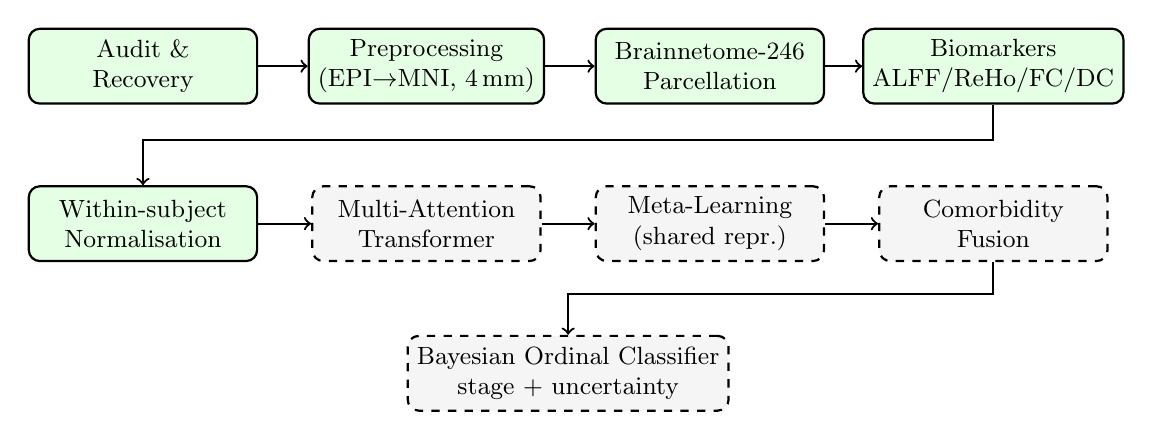
\begin{tikzpicture}[font=\small,node distance=0.35cm]
  \tikzset{
    blk/.style={rounded corners,thick,draw,minimum width=2.9cm,minimum height=0.95cm,
                align=center,fill=blue!8},
    dn/.style={blk,fill=green!10},
    pend/.style={blk,fill=gray!8,dashed},
    ar/.style={->,thick}
  }
  \node[dn] (a) at (0,0) {Audit \&\\Recovery};
  \node[dn] (b) at (3.6,0) {Preprocessing\\(EPI$\rightarrow$MNI, 4\,mm)};
  \node[dn] (c) at (7.2,0) {Brainnetome-246\\Parcellation};
  \node[dn] (d) at (10.8,0) {Biomarkers\\ALFF/ReHo/FC/DC};

  \node[dn] (e) at (0,-2.0) {Within-subject\\Normalisation};
  \node[pend] (f) at (3.6,-2.0) {Multi-Attention\\Transformer};
  \node[pend] (g) at (7.2,-2.0) {Meta-Learning\\(shared repr.)};
  \node[pend] (h) at (10.8,-2.0) {Comorbidity\\Fusion};

  \node[pend] (i) at (5.4,-3.9) {Bayesian Ordinal Classifier\\
                                 stage $+$ uncertainty};

  \draw[ar] (a) -- (b);
  \draw[ar] (b) -- (c);
  \draw[ar] (c) -- (d);
  \draw[ar] (d.south) -- ++(0,-0.45) -| (e.north);
  \draw[ar] (e) -- (f);
  \draw[ar] (f) -- (g);
  \draw[ar] (g) -- (h);
  \draw[ar] (h.south) -- ++(0,-0.4) -| (i.north);
\end{tikzpicture}
\caption{High-level architecture of the proposed system. Solid green blocks are
implemented and verified; dashed grey blocks are planned and not yet started.}
\label{fig:architecture}
\end{figure}

\section{Modules}

\subsection{Module 1: Data Audit, Recovery and Organisation}
\textbf{Purpose.} Establish a trustworthy cohort and an explicit record of what the
source data does and does not contain. \textbf{Inputs.} Raw ADNI DICOM archives and
partially converted NIfTI files. \textbf{Processing.} Inventory every acquisition;
locate acquisitions with metadata but no image data and convert them from DICOM;
detect duplicate and truncated acquisitions by checksum and header inspection; audit
slice-timing recoverability; organise into a BIDS-like layout with group membership
taken only from \texttt{participants.tsv}. \textbf{Outputs.} Organised cohort,
exclusion list, and audit reports. \textbf{Dependencies.} None.

\subsection{Module 2: Preprocessing}
\textbf{Purpose.} Bring every acquisition into a common template space with nuisance
signal suppressed. \textbf{Inputs.} Module~1 cohort. \textbf{Processing.} The eleven
steps of Table~\ref{tab:preproc}. \textbf{Outputs.} One preprocessed 4D BOLD volume,
brain mask, motion parameter file, nuisance design matrix, provenance record and QC
report per acquisition. \textbf{Dependencies.} Module~1.

\subsection{Module 3: Parcellation and Regional Time-Series Extraction}
\textbf{Purpose.} Reduce voxel-level data to a fixed 246-region representation.
\textbf{Inputs.} Preprocessed BOLD; original 2\,mm Brainnetome atlas.
\textbf{Processing.} Reorient the atlas losslessly, resample it onto each subject's
own BOLD grid using nearest-neighbour interpolation only, validate regional
coverage, and extract the mean BOLD time course of each region.
\textbf{Outputs.} Subject-aligned atlas, $T \times 246$ regional time-series matrix,
regional voxel counts and QC. \textbf{Dependencies.} Module~2.

\subsection{Module 4: Biomarker Generation}
\textbf{Purpose.} Derive the four complementary biomarkers.
\textbf{Inputs.} Preprocessed BOLD, aligned atlas, regional time series.
\textbf{Processing.} ALFF and ReHo are computed voxel-wise and then averaged within
each region; FC is computed between all region pairs; DC is derived from FC.
Definitions are given in Table~\ref{tab:biomarkers}.
\textbf{Outputs.} Per-acquisition biomarker vectors, the full connectivity matrix,
a combined regional feature matrix, and QC. \textbf{Dependencies.} Module~3.

\subsection{Module 5: Within-Subject Normalisation}
\textbf{Purpose.} Remove acquisition-level scaling that would otherwise dominate
cross-subject comparison. \textbf{Inputs.} Module~4 biomarkers.
\textbf{Processing.} Every statistic is computed from the acquisition's own 246
values, so the stage is leakage-free by construction. Methods are given in
Table~\ref{tab:norm}. \textbf{Outputs.} Normalised features in a separate directory
tree; raw biomarkers are never modified. \textbf{Dependencies.} Module~4.

\subsection{Module 6: Modelling and Evaluation (planned)}
\textbf{Purpose.} Learn the shared progression representation, fuse comorbidity, and
classify stage with uncertainty. \textbf{Inputs.} Module~5 features; cleaned
comorbidity table. \textbf{Processing.} Subject-grouped stratified
cross-validation, with cross-subject scaling fitted on training folds only;
multi-attention transformer; meta-learning across biomarkers; comorbidity fusion;
Bayesian ordinal classification; attention-based explanation.
\textbf{Outputs.} Stage predictions, uncertainty, region and biomarker attribution.
\textbf{Dependencies.} Modules~5 and~1.

\chapter{Implementation}\label{ch:impl}

All processing ran under WSL2 (Ubuntu) on Windows 11 with Python 3.12.3, NumPy
2.3.5, SciPy 1.15.3, NiBabel 5.4.2, Nilearn 0.14.1, ANTsPy 0.6.3, TemplateFlow
25.1.2 and FreeSurfer 7.4.1. Every long-running job used a single worker, with all
thread-count environment variables pinned to one.

\section{Module 1: Data Audit, Recovery and Organisation}

The initial audit covered 131 subjects and found 72 valid NIfTI files against 103
records that had JSON metadata but no image data at the audited location. Of these, 29
were recovered by converting raw DICOM archives (9 in the MCI group and 20 in the
SMC group, the latter representing 62.5\% of that group's final data), with no
conversion failures; the remaining records were reconciled against NIfTI files found
by the later per-group mapping audits. A dataset-wide checksum audit of 175 image files found no
orphans and exactly one hash collision, a subject exported twice under different
series numbers; the duplicate was excluded and the original retained. A second
acquisition was excluded for containing only 7 volumes where all others contain 140,
a truncation traced to the source export rather than to any processing step. Both
exclusions are recorded in a canonical exclusion list that every batch script
consults.

An early working note recorded six AD acquisitions as unrecoverable. This figure was
re-checked directly against the current source data before the production run and
found to be stale: all 20 AD subjects and all 25 AD acquisitions were present and
valid, and all were processed.

The slice-timing audit examined all 175 JSON sidecars and representative DICOM
headers spanning all 17 distinct protocol signatures in the archive, inspecting
private vendor groups as well as standard tags. No sidecar contained a
\texttt{SliceTiming} field. Within the DICOM headers, \texttt{AcquisitionTime} and
\texttt{TriggerTime} were identical across all slices sampled within a volume,
confirming volume-level rather than slice-level timing granularity. A Philips private
tag provides a per-slice \emph{spatial} index, but no tag anywhere states the
temporal acquisition order, and the spatial index was deliberately not used to infer
it. No multiband tag was found among decodable names. The audit's conclusion was
recorded as \texttt{SLICE\_TIMING\_NOT\_RECOVERABLE}, and no timing value was
inferred or fabricated at any point.

\section{Module 2: Preprocessing}\label{sec:preproc}

\begin{table}[H]
\centering
\caption{Implemented preprocessing pipeline.}
\label{tab:preproc}
\small
\begin{tabularx}{\textwidth}{@{}l>{\raggedright\arraybackslash}X@{}}
\toprule
\textbf{Step} & \textbf{Implementation} \\
\midrule
Input validation & 4D shape, all values finite, non-degenerate affine, TR $>0$,
non-empty image \\
Volume removal & First 5 volumes discarded for signal equilibration \\
Slice timing & \textbf{Not performed} --- not recoverable for this dataset \\
Motion correction & FreeSurfer~\cite{freesurfer} FS-FAST \texttt{mc-afni2}
(AFNI~\cite{afni} \texttt{3dvolreg}), rigid 6-DOF, reference = first retained frame;
native \texttt{.mcdat} preserved \\
Normalisation & Direct EPI-to-MNI152NLin6Asym via ANTsPy symmetric diffeomorphic
registration (\texttt{SyN})~\cite{ants}; no T1w exists, so the skull-stripped
temporal mean BOLD is registered to the template and the 4D series warped in a
single interpolation \\
Resampling & 4\,mm isotropic, continuous interpolation \\
Smoothing & 6\,mm FWHM Gaussian \\
Detrending & Per-voxel linear OLS; intercept and linear term removed, temporal mean
restored; no quadratic term \\
Nuisance regression & 27 regressors in every acquisition: intercept, Friston-24~\cite{friston24},
white-matter signal from a population template prior, and global signal. A CSF
candidate from the same priors failed its reliability gate in all 165 acquisitions \\
Band-pass filter & 0.01--0.10\,Hz, 2nd-order Butterworth, zero-phase
\texttt{filtfilt}; Nyquist validity checked per acquisition \\
QC & tSNR, SNR, framewise displacement~\cite{fd}, DVARS, spatial and temporal
entropy \\
\bottomrule
\end{tabularx}
\end{table}

Two implementation points deserve emphasis. First, because no T1w image exists,
white-matter and CSF candidate regressors are derived from published population
tissue probability priors rather than from subject-specific segmentation; a candidate
is included only if its mask retains at least 20 voxels and its correlation with the
global signal is below 0.98 in magnitude. The white-matter regressor passed this gate
in all 165 acquisitions and the CSF regressor failed it in all 165, so the nuisance
design matrix has exactly 27 columns in every acquisition (intercept, 24 Friston
terms, white matter, global signal); every provenance record states
\texttt{CSF\_status = NOT PERFORMED}. The ventricular CSF prior is too thin to survive
at 4\,mm: the corresponding 2\,mm pilot mask held only 111 voxels (888\,mm$^3$)
after thresholding at 0.90 and intersection with the brain mask, which is roughly 14
voxels on the 4\,mm grid, below the 20-voxel minimum. The voxel count and correlation
at the gate were not stored per acquisition, so this is the explanation consistent
with the logged evidence rather than a per-acquisition measurement. No substitute
CSF regressor was introduced. Second, contrast-to-noise ratio is reported as not reliably
computable for all 165 acquisitions, because it requires a tissue segmentation this
dataset cannot provide (no T1w image exists for any of the 131 subjects); no
segmentation was fabricated to produce a number.

The band-pass step validates, per acquisition, that the requested upper cutoff lies
below the Nyquist frequency implied by that acquisition's own TR. Eight acquisitions
failed this check. All eight share a TR of approximately 6.02\,s, roughly double the
3.0\,s used elsewhere in the cohort, giving a Nyquist limit near 0.083\,Hz --- below
the 0.10\,Hz cutoff. These were refused rather than silently reprocessed with an
altered band, since changing the filter for a subset would make those acquisitions
non-comparable with the rest. Seven of the eight have a TR of 6.02158\,s and one has
6.02353\,s; all eight belong to site~002 (subject identifiers \texttt{002\_S\_xxxx}).

\section{Module 3: Parcellation and Regional Time-Series Extraction}

The Brainnetome atlas~\cite{brainnetome} is supplied at 2\,mm in LAS orientation
whereas the
preprocessed BOLD is RAS, so the atlas is first reoriented to canonical orientation,
a lossless array operation involving no interpolation, verified by per-label voxel
count equality. It is then resampled onto each subject's own BOLD grid using
\emph{nearest-neighbour interpolation only}. This is essential: atlas values are
categorical region identifiers, and linear or spline interpolation would produce
fractional labels with no meaning. Regional time series are extracted by direct index
masking on the verified-identical grid rather than through a masker utility that
might silently re-resample the labels a second time.

\section{Module 4: Biomarker Generation}

\begin{table}[H]
\centering
\caption{Implemented biomarker definitions.}
\label{tab:biomarkers}
\small
\begin{tabularx}{\textwidth}{@{}l>{\raggedright\arraybackslash}Xl@{}}
\toprule
\textbf{Biomarker} & \textbf{Definition as implemented} & \textbf{Shape} \\
\midrule
ALFF & Mean FFT amplitude within 0.01--0.10\,Hz of the mean-centred voxel time
series, then averaged within each region & $(246,)$ \\
ReHo & Kendall's coefficient of concordance over a 27-voxel $3\times3\times3$
neighbourhood including the centre voxel, with the neighbour count reduced at the
mask boundary, then averaged within each region & $(246,)$ \\
FC & Pearson correlation between all region pairs; signed, unthresholded, diagonal
retained & $(246,246)$ \\
DC & $DC_i = \sum_{j \neq i} FC_{ij}$; weighted, signed, unthresholded,
self-connection excluded & $(246,)$ \\
\bottomrule
\end{tabularx}
\end{table}

ALFF and ReHo are computed at voxel level and only then aggregated to regions,
rather than computed from the regional time series, so that local spatial
information is used where the definitions require it. The 27-voxel ReHo neighbourhood
is the original formulation~\cite{reho} and the default of established toolboxes,
chosen for comparability rather than arbitrarily. Because the preprocessed BOLD has already been
band-pass filtered, ALFF is computed on an already band-limited spectrum; this is a
documented consequence of the fixed pipeline rather than a change of method.

The connectivity matrix is retained in full. No threshold, binarisation or absolute
value is applied, and negative correlations are preserved, since thresholding would
impose an unvalidated choice and discard the sign information that distinguishes
anti-correlated from unconnected regions.

A single-acquisition pilot was implemented and validated first. Before scaling to the
cohort, the production implementation was required to reproduce that pilot: ALFF,
ReHo, regional time series, atlas labels and regional voxel counts were recovered
bit-identically, and FC and DC agreed to within $1.8 \times 10^{-15}$. Only then was
the pilot's own output directory protected and the remaining acquisitions processed.

\section{Module 5: Within-Subject Normalisation}

\begin{table}[H]
\centering
\caption{Within-subject normalisation, computed from each acquisition's own 246
regional values only.}
\label{tab:norm}
\small
\begin{tabularx}{\textwidth}{@{}l>{\raggedright\arraybackslash}X@{}}
\toprule
\textbf{Feature} & \textbf{Transform and rationale} \\
\midrule
mALFF & $\mathrm{ALFF}_i / \overline{\mathrm{ALFF}}$. Raw ALFF is in FFT amplitude units
proportional to raw BOLD intensity and spans roughly $8.5\times10^{2}$ to
$2.2\times10^{5}$ across acquisitions; the ratio removes this
scaling~\cite{falff}. A ratio is used rather than a $z$-score because ALFF is
strictly positive \\
mReHo & $\mathrm{ReHo}_i / \overline{\mathrm{ReHo}}$, removing each subject's global
coherence offset \\
DC$_z$ & $(\mathrm{DC}_i - \overline{\mathrm{DC}}) / \sigma_{\mathrm{DC}}$ with
$\mathrm{ddof}=0$~\cite{centrality}. A $z$-score is used because DC is signed, which
rules out min--max scaling \\
Fisher-$z$ FC & $\mathrm{arctanh}\big(\mathrm{clip}(r,\pm0.999999)\big)$ on
off-diagonal entries, variance stabilising the correlations. The diagonal is zeroed
\emph{before} the transform so that $\mathrm{arctanh}(1)=\infty$ is never produced,
then set to exactly zero; negative correlations stay negative \\
\bottomrule
\end{tabularx}
\end{table}

\textbf{Leakage-free by construction.} Every statistic in Table~\ref{tab:norm} is
computed from that acquisition's own 246 values. No cross-subject statistic and no
diagnostic label is used at any point, so the stage cannot carry information from a
test subject into training. Cross-subject scaling is deliberately deferred to the
modelling stage, where it will be fitted on training folds only. Outputs are written
to a separate directory tree, and the script refuses any write path inside a raw
\texttt{biomarkers} directory.

\begin{table}[H]
\centering
\caption{Verification of within-subject normalisation (165 acquisitions, 0 failures).}
\label{tab:normcheck}
\small
\begin{tabularx}{\textwidth}{@{}>{\raggedright\arraybackslash}Xr@{}}
\toprule
\textbf{Check} & \textbf{Result} \\
\midrule
Acquisitions normalised; failures & 165 / 165; 0 \\
Non-finite values in inputs; in outputs & 0; 0 \\
mean(mALFF) and mean(mReHo) per acquisition & 1.000000 in all 165 \\
mean(DC$_z$), largest magnitude & $\leq 1.6\times10^{-16}$ \\
std(DC$_z$) per acquisition & 1.000000 in all 165 \\
Fisher-$z$ diagonal exactly zero & 165 / 165 \\
Fisher-$z$ maximum asymmetry & $5.329\times10^{-15}$ \\
Negative correlations preserved as negative & 165 / 165 \\
Off-diagonal entries requiring clipping at $\pm0.999999$ & 0 \\
Fisher-$z$ range across the dataset & $-2.2653$ to $2.5924$ \\
\bottomrule
\end{tabularx}
\end{table}

\section{Feature Redundancy: FC Strength and DC}\label{sec:redundancy}

Auditing our own features, rather than inheriting them from the design, exposed an
exact redundancy. The pipeline stores a regional connectivity strength defined as the
\emph{mean} of each region's off-diagonal connectivity, while DC is the \emph{sum}
over the same 245 entries, so
\[
  \mathrm{FCS}_i \;=\; \frac{1}{245}\sum_{j\neq i}\mathrm{FC}_{ij}
  \;=\; \frac{\mathrm{DC}_i}{245}.
\]
Table~\ref{tab:redundancy} gives the measurements.

\begin{table}[H]
\centering
\caption{Measured equivalence of FC\_Strength and DC.}
\label{tab:redundancy}
\small
\begin{tabularx}{\textwidth}{@{}>{\raggedright\arraybackslash}Xr@{}}
\toprule
\textbf{Comparison} & \textbf{Result} \\
\midrule
Raw outputs, all 165 acquisitions: $\max|\mathrm{DC}/245-\mathrm{FCS}|$ & $6.939\times10^{-18}$ \\
Raw outputs: minimum Pearson $r$ across acquisitions & $1.000000000000$ \\
Stage matrices (both within-subject $z$-scored): $\max|\mathrm{DC}_z-\mathrm{FCS}_z|$ & $6.661\times10^{-16}$ \\
Stage matrices: Pearson $r$ & $1.0$ \\
\bottomrule
\end{tabularx}
\end{table}

Under any scale-invariant normalisation the two columns become numerically identical.

\textbf{Design correction.} Review~I specified a $246\times4$ regional feature matrix
(ALFF, ReHo, DC, FC strength). One column was a deterministic rescaling of another,
so the independent regional features are three. The corrected model input is a
$246\times3$ regional matrix (mALFF, mReHo, DC$_z$) \emph{plus} the full
$246\times246$ Fisher-$z$ connectivity matrix. FC is not dropped: it moves from a
collapsed per-region scalar into its full matrix form, which carries strictly more
information. The raw FC strength files are retained unaltered; only the model feature
set changes. This is a correction derived from auditing the features, not a pipeline
error.

\section{Engineering for an Unstable Execution Environment}

Early production runs failed repeatedly, and diagnosis of the failure mode
materially shaped the implementation. The symptom was that the virtual machine
terminated after roughly five to twelve acquisitions with no Python traceback. The
cause was sustained small-granularity array input/output against the Windows
drive mount, which produced \texttt{Errno 5} input/output errors and virtual machine
level failures under load. Three changes resolved it. Each acquisition is now staged
on the native Linux filesystem and its results copied to the Windows-visible tree
only once complete, so a crash never leaves a partially written output directory.
Resume validation reads array shapes through memory mapping and file headers instead
of loading every finished acquisition back into memory, which had been re-reading
gigabytes on every restart. Finally, a wrapper distinguishes a genuine Python error,
which stops the run for inspection, from a virtual machine failure, which triggers a
restart and resumption from the last validated checkpoint. Restart count fell from
23 to 2 for the same workload.

Checkpointing re-validates the actual files on disk --- shapes, finiteness and
structural invariants --- before treating any acquisition as complete, so the
checkpoint record alone is never trusted.

\chapter{Results and Discussion}

\section{Cohort Composition}

\begin{table}[H]
\centering
\caption{Cohort composition after audit, recovery and exclusion, listed in
progression order.}
\label{tab:cohort}
\small
\begin{tabular}{lrrrr}
\toprule
\textbf{Stage} & \textbf{Eligible} & \textbf{Preprocessed} & \textbf{Biomarkers} &
\textbf{Subjects} \\
\midrule
CN (CN\_Final)   & 29 & 27 & 27 & 26 \\
SMC (SMC\_Final) & 32 & 31 & 31 & 21 \\
EMCI      & 30 & 29 & 29 & 26 \\
MCI       & 35 & 32 & 32 & 14 \\
LMCI      & 22 & 21 & 21 & 20 \\
AD        & 25 & 25 & 25 & 20 \\
\midrule
\textbf{Total} & \textbf{173} & \textbf{165} & \textbf{165} & \textbf{127} \\
\bottomrule
\end{tabular}
\end{table}

Table~\ref{tab:cohort} reports the figure that most constrains the modelling stage.
The 165 acquisitions derive from only 127 distinct subjects: 96 subjects contribute
one acquisition, 25 contribute two, 5 contribute three and 1 contributes four. The
MCI group illustrates why this matters. By acquisition count it is the largest group
at 35, but it comprises only 14 subjects, at 2.3 acquisitions per subject. Because
validation splits must group by subject --- otherwise the same individual appears in
both training and test data --- 14 is the number that bounds what can be claimed
about that class. No subject appears in more than one group, so labels are
subject-consistent.

\section{Preprocessing Quality Control}\label{sec:qc}

Table~\ref{tab:groupqc} summarises acquisition-level quality control by stage. One
acquisition is treated separately and is flagged explicitly.

\begin{table}[H]
\centering
\caption{Preprocessing quality control by stage. All columns except the last exclude
the single artifact acquisition described below ($n=164$ overall). The raw tSNR mean as
originally reported by the dataset audit, which includes it, is shown in the last
column.
FD is mean framewise displacement in mm; ``med.'' is the median.}
\label{tab:groupqc}
\footnotesize
\setlength{\tabcolsep}{4pt}
\begin{tabular}{@{}lrrrrrr@{}}
\toprule
\textbf{Stage} & \textbf{$n$} & \textbf{tSNR mean} & \textbf{tSNR med.} &
\textbf{SNR mean} & \textbf{FD mean} & \textbf{tSNR raw} \\
\midrule
CN (CN\_Final) & 26 & 131.63 & 132.58 & 12.95 & 0.352 & \textbf{12064.36} \\
SMC (SMC\_Final) & 31 & 125.71 & 123.70 & 13.15 & 0.375 & 125.71 \\
EMCI & 29 & 137.49 & 133.16 & 13.76 & 0.355 & 137.49 \\
MCI & 32 & 137.05 & 139.24 & 12.94 & 0.321 & 137.05 \\
LMCI & 21 & 127.54 & 121.41 & 12.99 & 0.322 & 127.54 \\
AD & 25 & 114.06 & 118.76 & 13.49 & 0.439 & 114.06 \\
\midrule
\textbf{All} & \textbf{164} & \textbf{129.40} & \textbf{127.95} & \textbf{13.22} &
\textbf{0.360} & 2082.04 \\
\bottomrule
\end{tabular}
\end{table}

Dataset-wide medians over the 164 acquisitions are tSNR 127.95, SNR 13.12, mean
framewise displacement 0.317\,mm and raw-intensity DVARS 15270. Contrast-to-noise
ratio is not available (N/A) for all 165 acquisitions, since no T1w image exists for
any of the 131 subjects. Head motion is substantial: 134 of the 164 acquisitions
exceed 0.2\,mm mean FD, 90 exceed 0.3\,mm and 28 exceed 0.5\,mm. High motion is
flagged, not excluded, under the frozen processing policy, so motion will enter the
modelling stage as a covariate.

\textbf{Artifact acquisition (reported, not silently dropped).} The audit-reported
CN tSNR mean of 12064 is produced by a single acquisition,
\texttt{CN\_Final/\allowbreak sub-018S4313/\allowbreak ses-01/\allowbreak run-01}, whose tSNR is 322,315 against a
dataset median of 128. The ratio is mean over standard deviation per voxel, so
near-zero-variance voxels inflate it; the project methodology record attributes the
value to this effect. The same acquisition has mean FD 1.079\,mm (among the four
highest of 165) and an anomalously low spatial entropy of 4.21 bits against a
cohort mean of 7.18 for the other 164. It is excluded from the tSNR, SNR, FD and
DVARS summaries in Table~\ref{tab:groupqc} and from the medians above, and the raw
value is kept visible in the last column. With it removed, the CN tSNR mean is 131.63
(median 132.58), in line with the other stages. The acquisition itself remains among the 165
preprocessed acquisitions and in every downstream count; how it is handled in
modelling has not yet been decided.

\section{Biomarker Quality}

\begin{table}[H]
\centering
\caption{Dataset-level quality control over all 165 processed acquisitions.}
\label{tab:qc}
\small
\begin{tabularx}{\textwidth}{@{}>{\raggedright\arraybackslash}Xr@{}}
\toprule
\textbf{Check} & \textbf{Result} \\
\midrule
Acquisitions with complete biomarker outputs & 165 / 165 \\
Processing failures at the biomarker stage & 0 \\
Brainnetome coverage 246/246 regions & 165 / 165 \\
Regions with zero voxels (any acquisition) & 0 \\
Smallest region, across the whole dataset & 10 voxels \\
Regional time-series matrices of shape $(135,246)$ & 165 / 165 \\
Non-finite values in regional time series & 0 \\
Regions with zero temporal variance & 0 \\
ALFF: non-finite or negative values & 0 \\
ReHo: values outside the valid $[0,1]$ range & 0 \\
ReHo range across dataset & 0.2352--0.8231 \\
FC: non-finite values & 0 \\
FC maximum diagonal error & $2.2\times10^{-16}$ \\
FC maximum asymmetry & $2.2\times10^{-16}$ \\
DC recomputed independently from stored FC, max.\ difference &
$0.0\times10^{0}$ \\
Acquisitions passing all cross-file consistency checks & 165 / 165 \\
\bottomrule
\end{tabularx}
\end{table}

The result in Table~\ref{tab:qc} that carries the most evidential weight is the
independent recomputation of degree centrality. For every acquisition, DC was
recomputed from the stored connectivity matrix in a separate process that read only
saved files, and compared against the stored vector; the maximum difference across
all 165 acquisitions was exactly zero. This verifies not merely that the files are
well formed but that the stored values are the ones the documented definition
produces.

Complete 246/246 regional coverage in every acquisition follows from the pipeline
design: because all acquisitions are registered to the same template-derived 4\,mm
grid, the aligned atlas is identical across the cohort. This was nonetheless
verified per acquisition rather than assumed.

Normalisation was applied to all 165 acquisitions with no failures
(Table~\ref{tab:normcheck}). Mean mALFF and
mean mReHo equal 1.000000 for every acquisition; DC$_z$ has mean below
$1.6\times10^{-16}$ and standard deviation 1.000000; the Fisher-$z$ connectivity
matrix is symmetric to $5.3\times10^{-15}$ with a diagonal of exactly zero in all
165 cases. No off-diagonal correlation anywhere in the dataset exceeded the
$\pm0.999999$ clipping bound, so that safeguard never engaged --- confirming no
region pair is numerically perfectly correlated.

\section{Stage-wise Group Patterns: A Negative Univariate Result}\label{sec:heatmaps}

We tested whether a univariate, per-region group-mean signal distinguishes the six
progression stages. Stage-wise matrices of size $246\times6$ were generated for
mALFF, mReHo, DC$_z$ and FC\_Strength with subject-level aggregation: acquisitions
were averaged within subject first and subjects then averaged within stage, so each
of the 127 subjects counts once although there are 165 acquisitions. The subject
counts are CN 26, SMC 21, EMCI 26, MCI 14, LMCI 20 and AD 20. Each region was then
$z$-scored across the six stages so that colour shows how a region changes across
stages and not how large it is (Figure~\ref{fig:heatmaps}). The absolute-value
versions (\texttt{derivatives/\allowbreak STAGE\_HEATMAPS/\allowbreak *\_absolute.png}) are available but
are not shown, because they are dominated by anatomical differences between regions.

\begin{figure}[H]
\centering
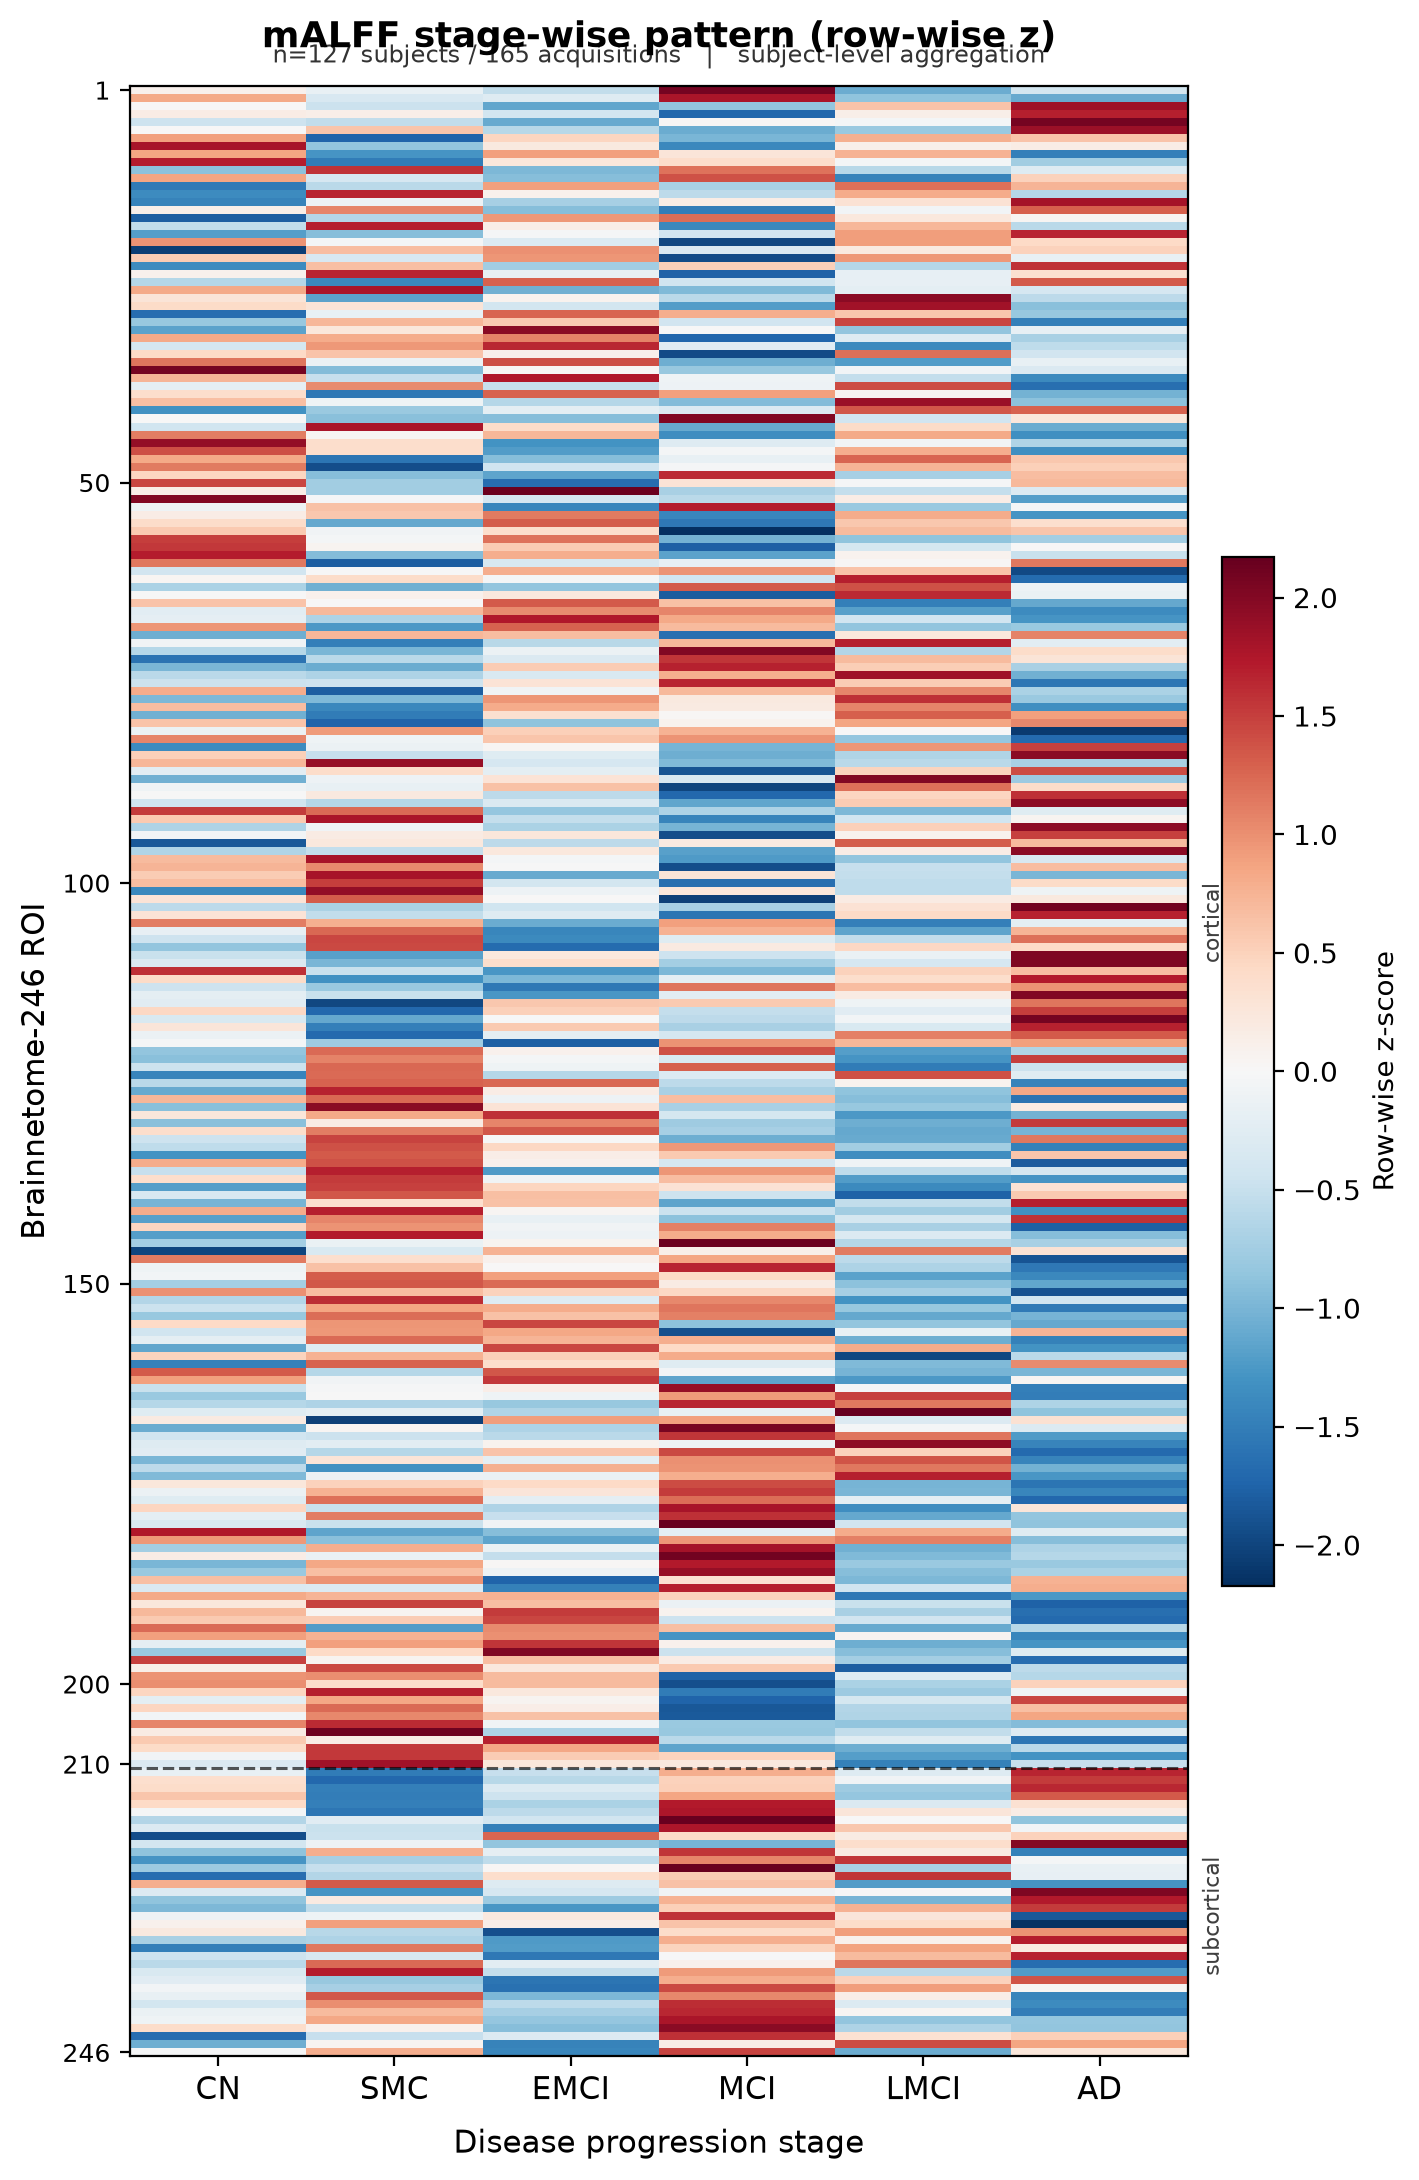
\includegraphics[width=0.31\textwidth]{figures/mALFF_rowz.png}\hfill
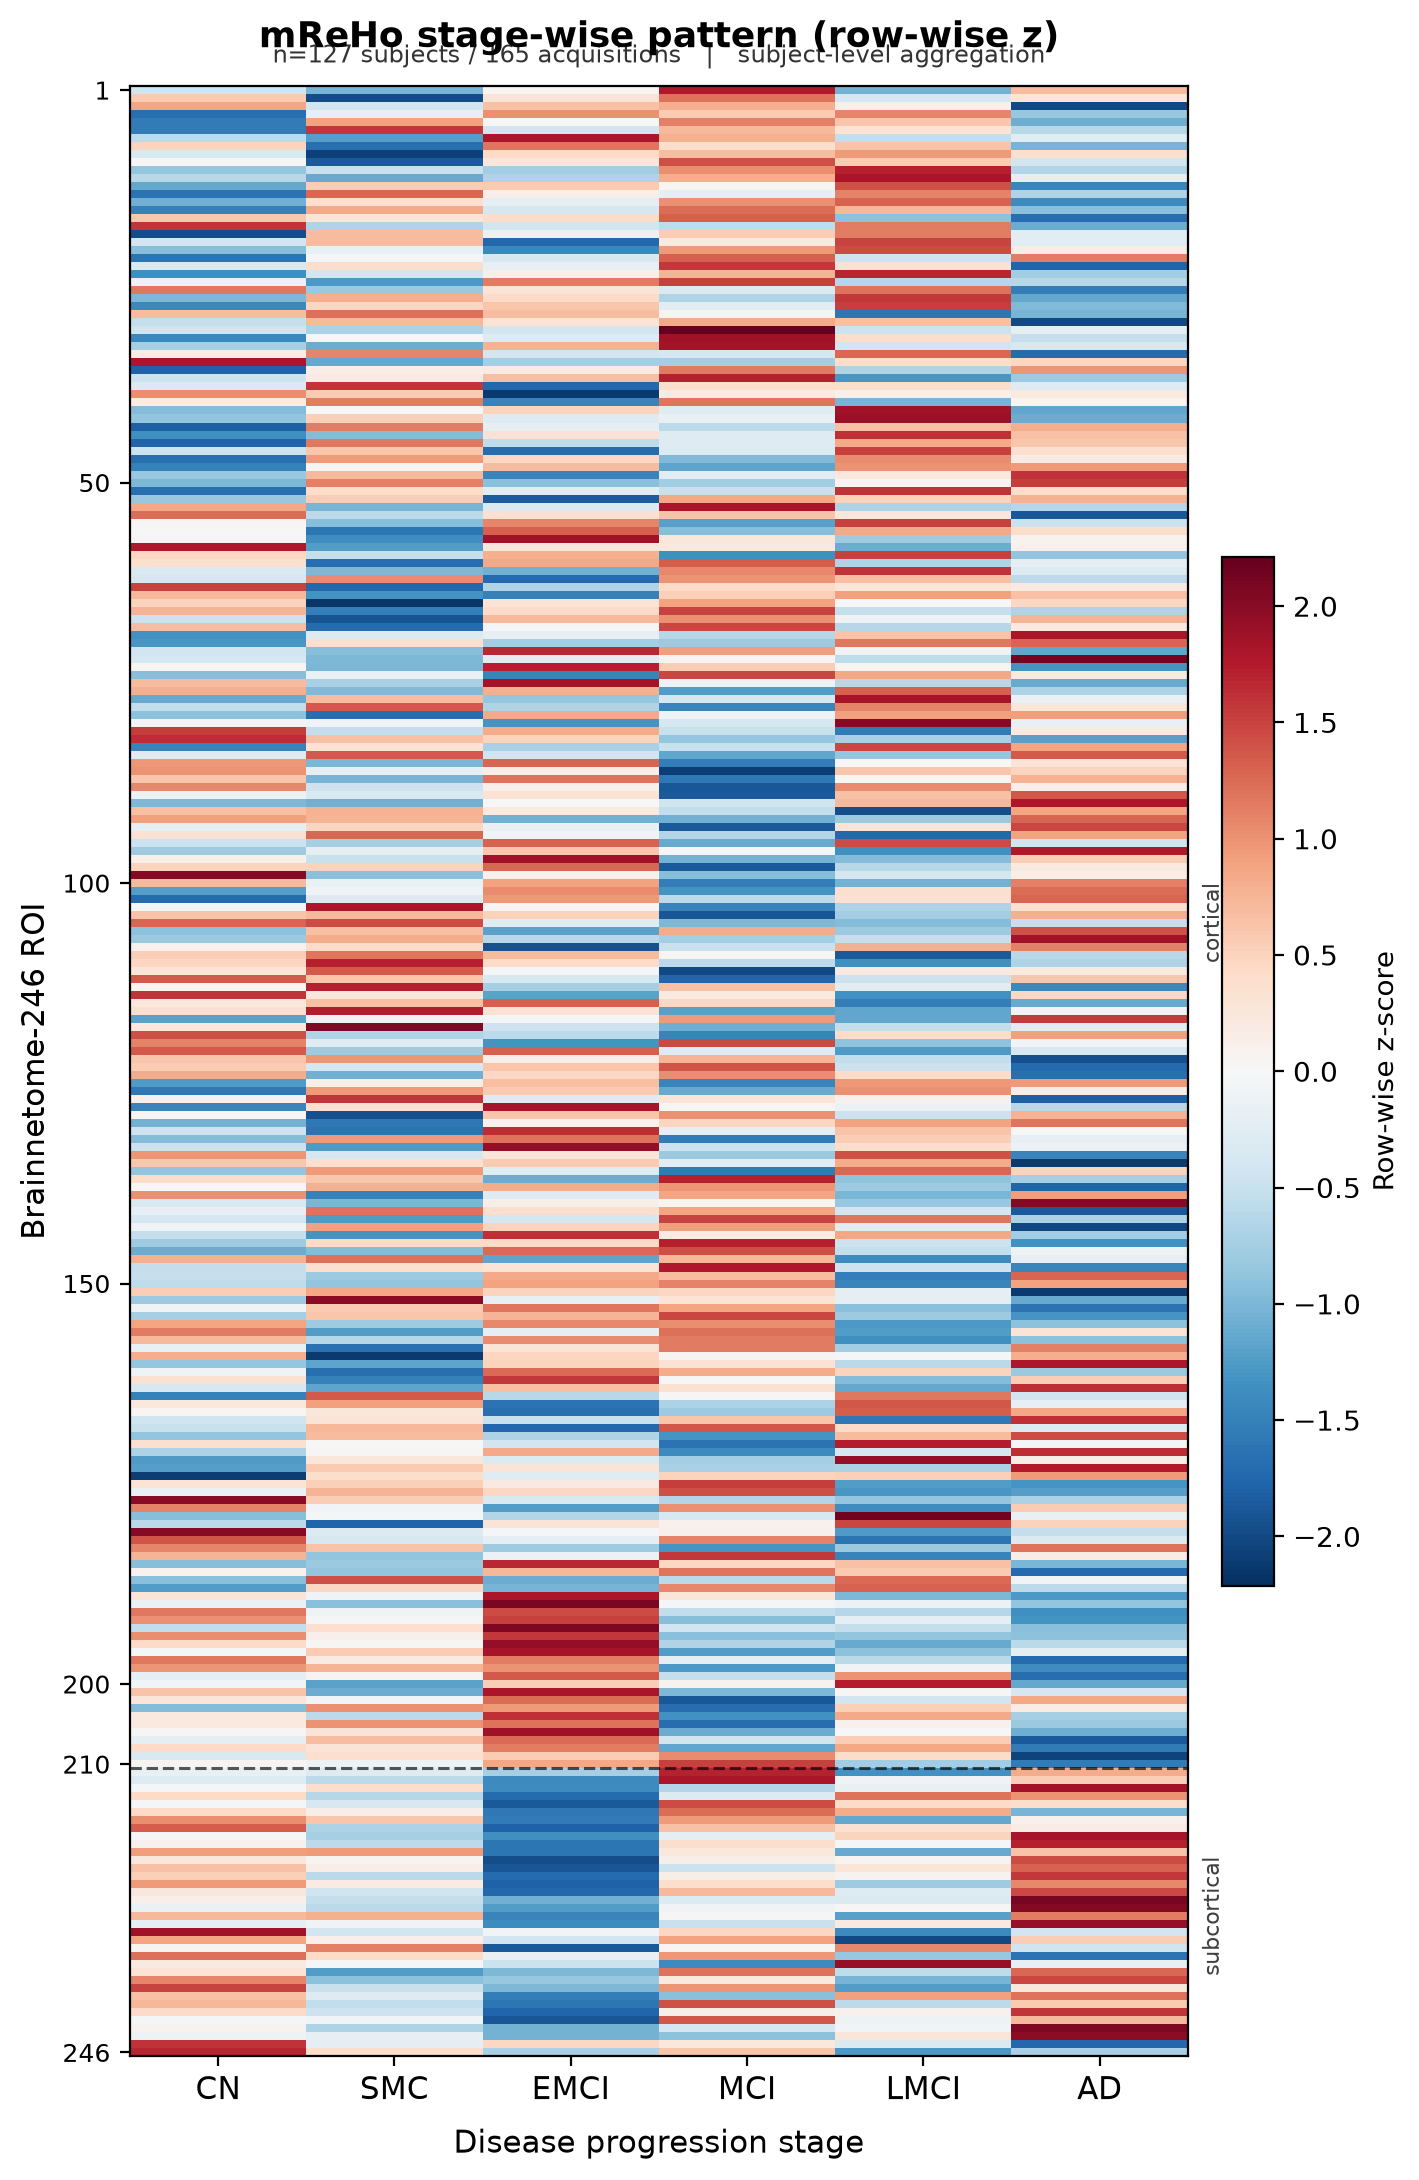
\includegraphics[width=0.31\textwidth]{figures/mReHo_rowz.png}\hfill
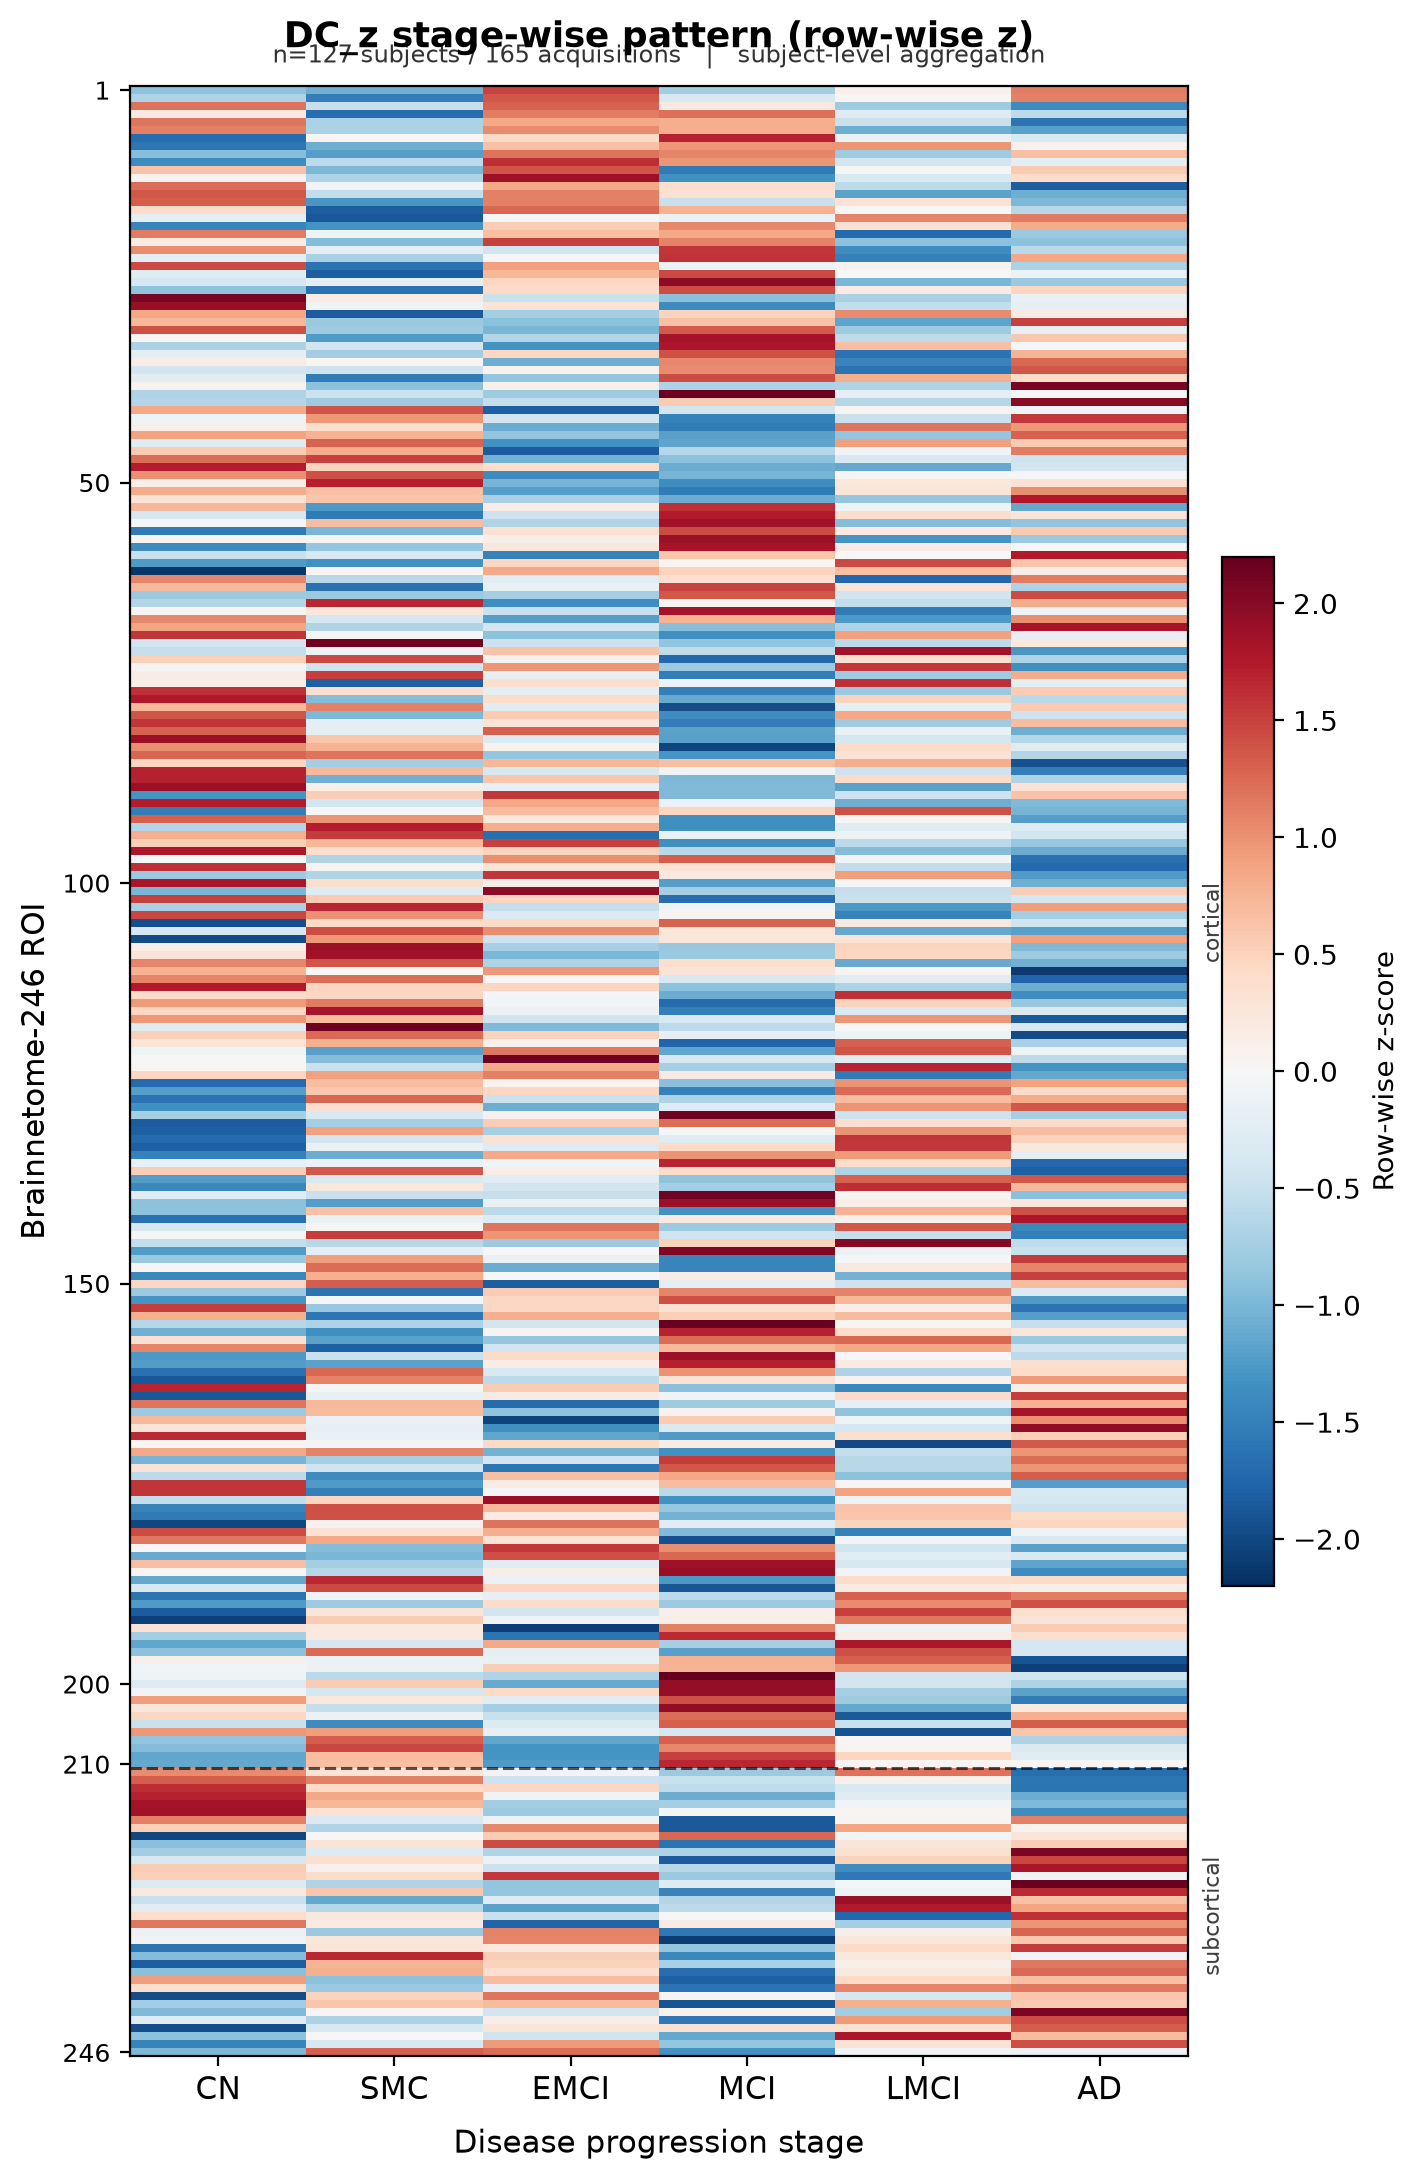
\includegraphics[width=0.31\textwidth]{figures/DC_z_rowz.png}
\caption{Stage-wise regional biomarker patterns across the six-stage progression
(CN, SMC, EMCI, MCI, LMCI, AD) for 127 subjects; from left to right mALFF, mReHo
and DC$_z$. Rows are the 246 Brainnetome ROIs in atlas order (cortical 1--210 above
the dashed line, subcortical 211--246 below); columns are progression stages. Each
ROI is $z$-scored independently across the six stages, so colour encodes how a
region changes across stages rather than its absolute magnitude. Acquisitions were
averaged within subject before averaging across subjects, so each of the 127
subjects contributes once. These are descriptive, exploratory visualisations; they
do not demonstrate disease progression and no statistical testing was performed.}
\label{fig:heatmaps}
\end{figure}

\begin{table}[H]
\centering
\caption{Monotonic trends in the stage means. A region counts as monotonic if its
six stage means increase, or decrease, strictly from CN to AD. The expectation by
chance is $246\times2/6!\approx0.7$, the combinatorial value when the six stage
means of a region are exchangeable; it is not a hypothesis test. The last column is
the median over regions of the standard deviation of the six stage means, divided by
the standard deviation across regions of the per-region mean (population
standard deviations).}
\label{tab:monotonic}
\small
\begin{tabularx}{\textwidth}{@{}l>{\centering\arraybackslash}X>{\centering\arraybackslash}X>{\centering\arraybackslash}X@{}}
\toprule
\textbf{Biomarker} & \textbf{ROIs with monotonic CN$\rightarrow$AD trend} &
\textbf{Expected by chance} & \textbf{Stage SD / between-ROI SD} \\
\midrule
mALFF & 1 / 246 (decreasing) & $\approx0.7$ & 0.18 \\
mReHo & 0 / 246 & $\approx0.7$ & 0.24 \\
DC$_z$ & 1 / 246 (increasing) & $\approx0.7$ & 0.23 \\
\bottomrule
\end{tabularx}
\end{table}

The result (Table~\ref{tab:monotonic}) is negative and is reported as such, in four steps.
\begin{enumerate}[label=\arabic*.]
  \item We tested for a univariate, per-region group-mean progression signal.
  \item It is not detectable. Only 1, 0 and 1 of 246 regions are monotonic from CN to
        AD, which is no more than the roughly 0.7 that chance alone gives, and the
        variation across stages is about 4--5 times smaller than the anatomical
        variation between regions (ratios 0.18--0.24).
  \item This is informative, not a failure of the pipeline. Per-region stage means
        discard the entire $246\times246$ connectivity structure, and they can only
        reveal effects large enough to survive averaging over 14--26 subjects per
        stage. The result does not show that the biomarkers carry no stage
        information; it shows that group means of single regions do not expose it.
  \item The multivariate architecture is therefore motivated and not assumed: the
        transformer sees each subject individually and all 246 regions jointly, with
        connectivity intact.
\end{enumerate}
No heatmap in this report is evidence of progression, and the pipeline has not been
tested on any classification task.

Figure~\ref{fig:redundancy} places the DC$_z$ and FC\_Strength heatmaps side by
side, which turns the redundancy of Section~\ref{sec:redundancy} into a visual proof.

\begin{figure}[H]
\centering
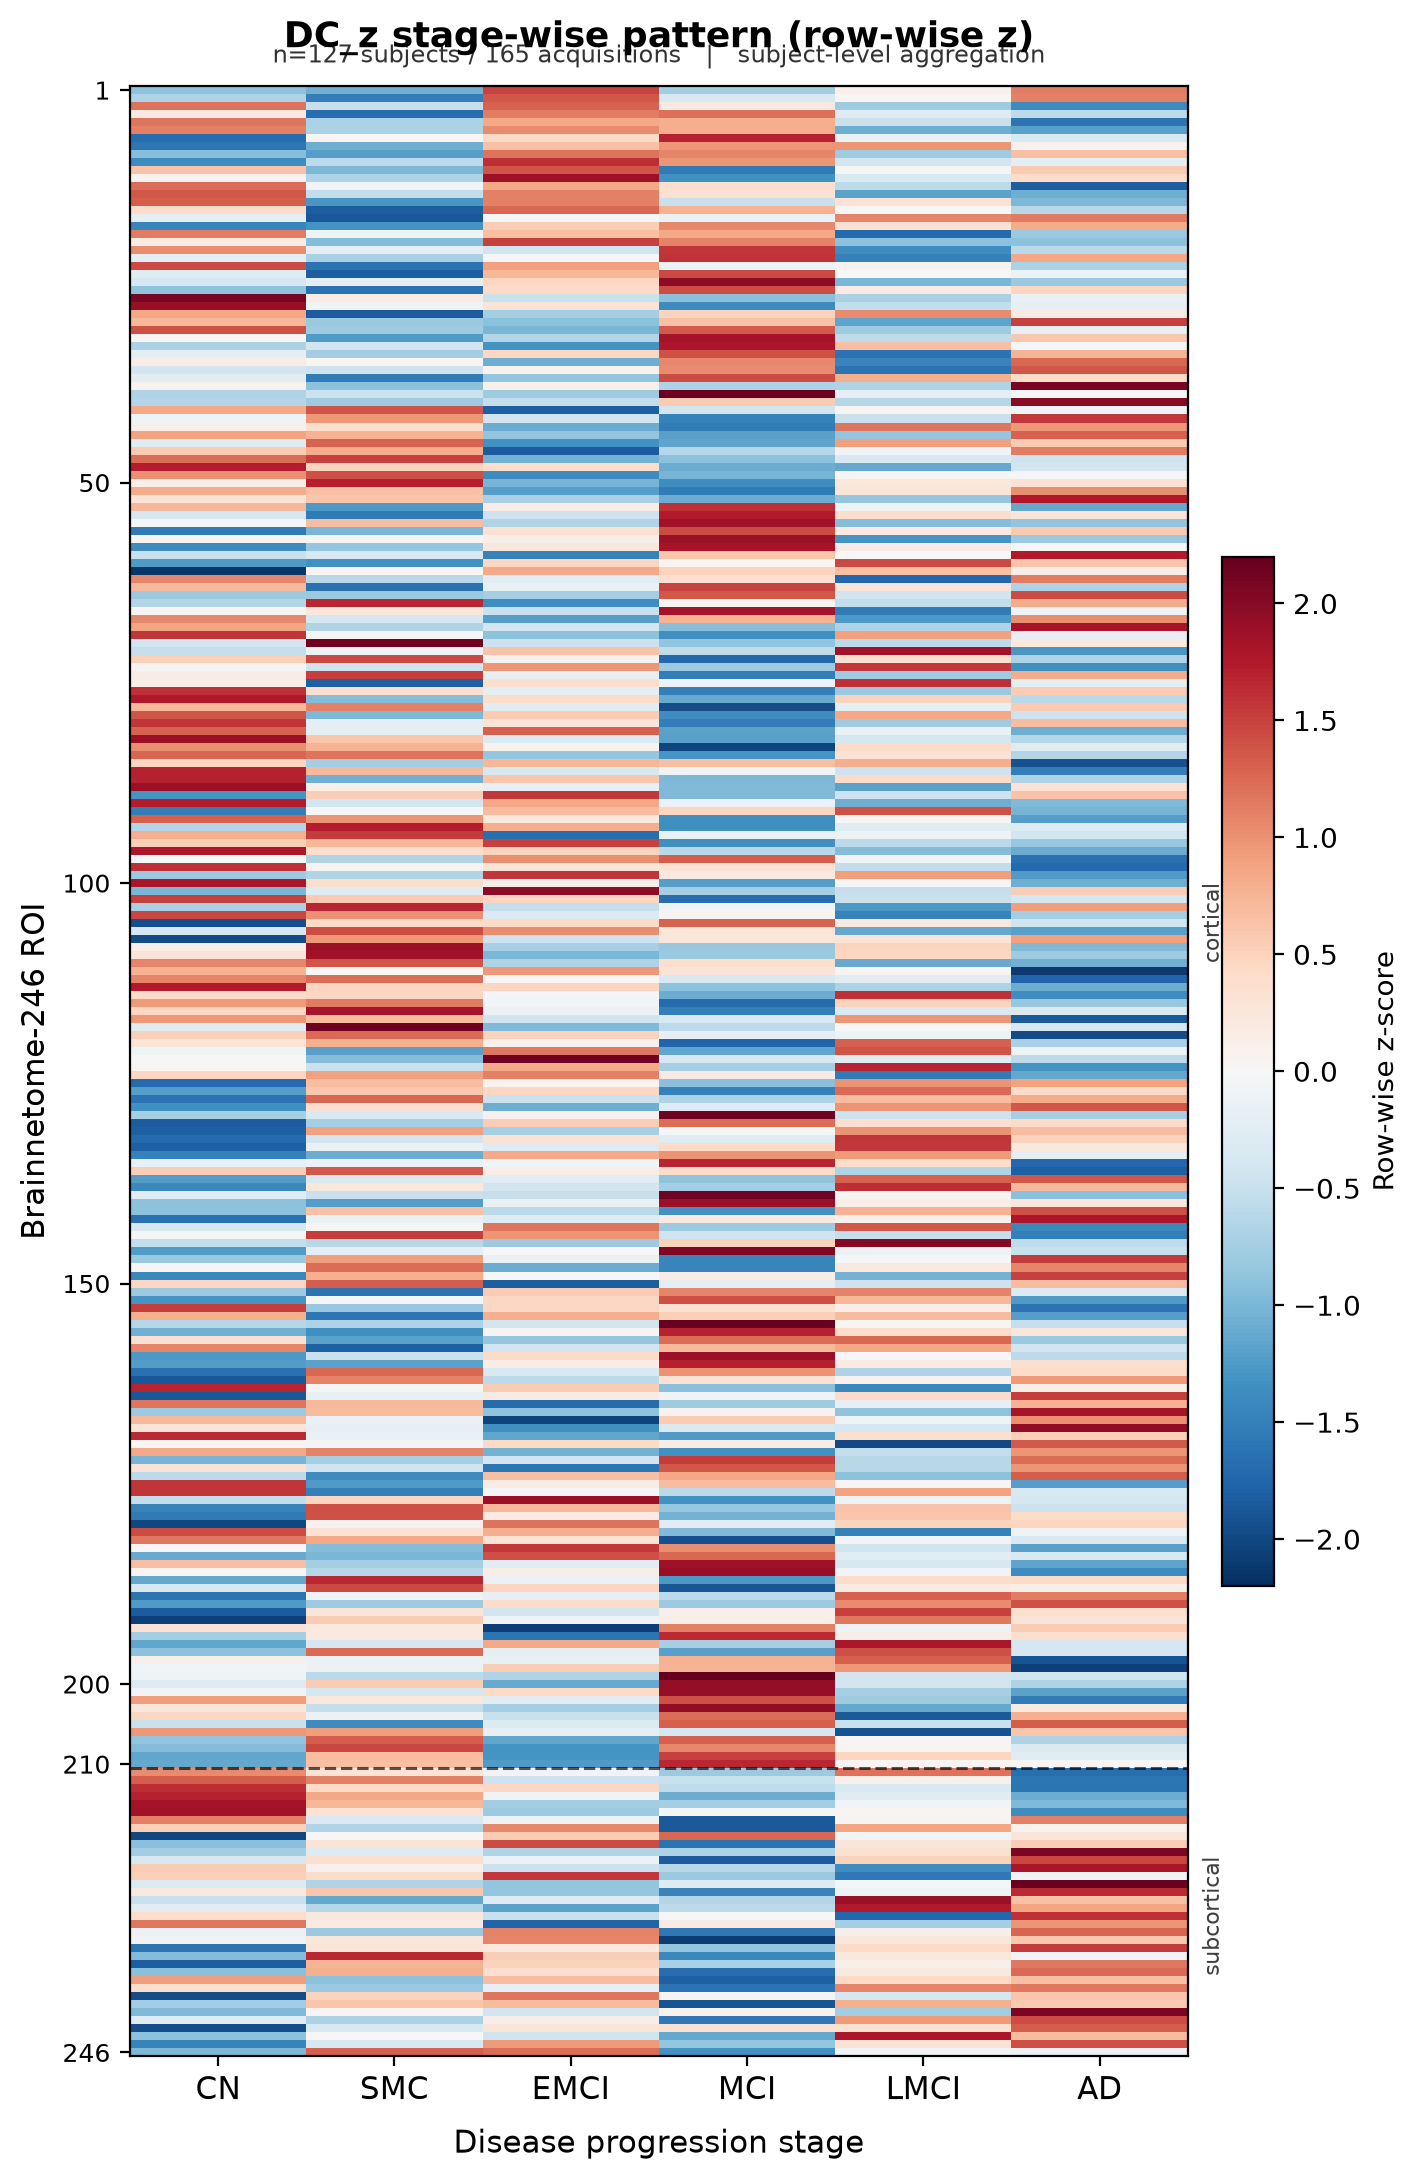
\includegraphics[height=0.44\textheight,keepaspectratio]{figures/DC_z_rowz.png}\hfill
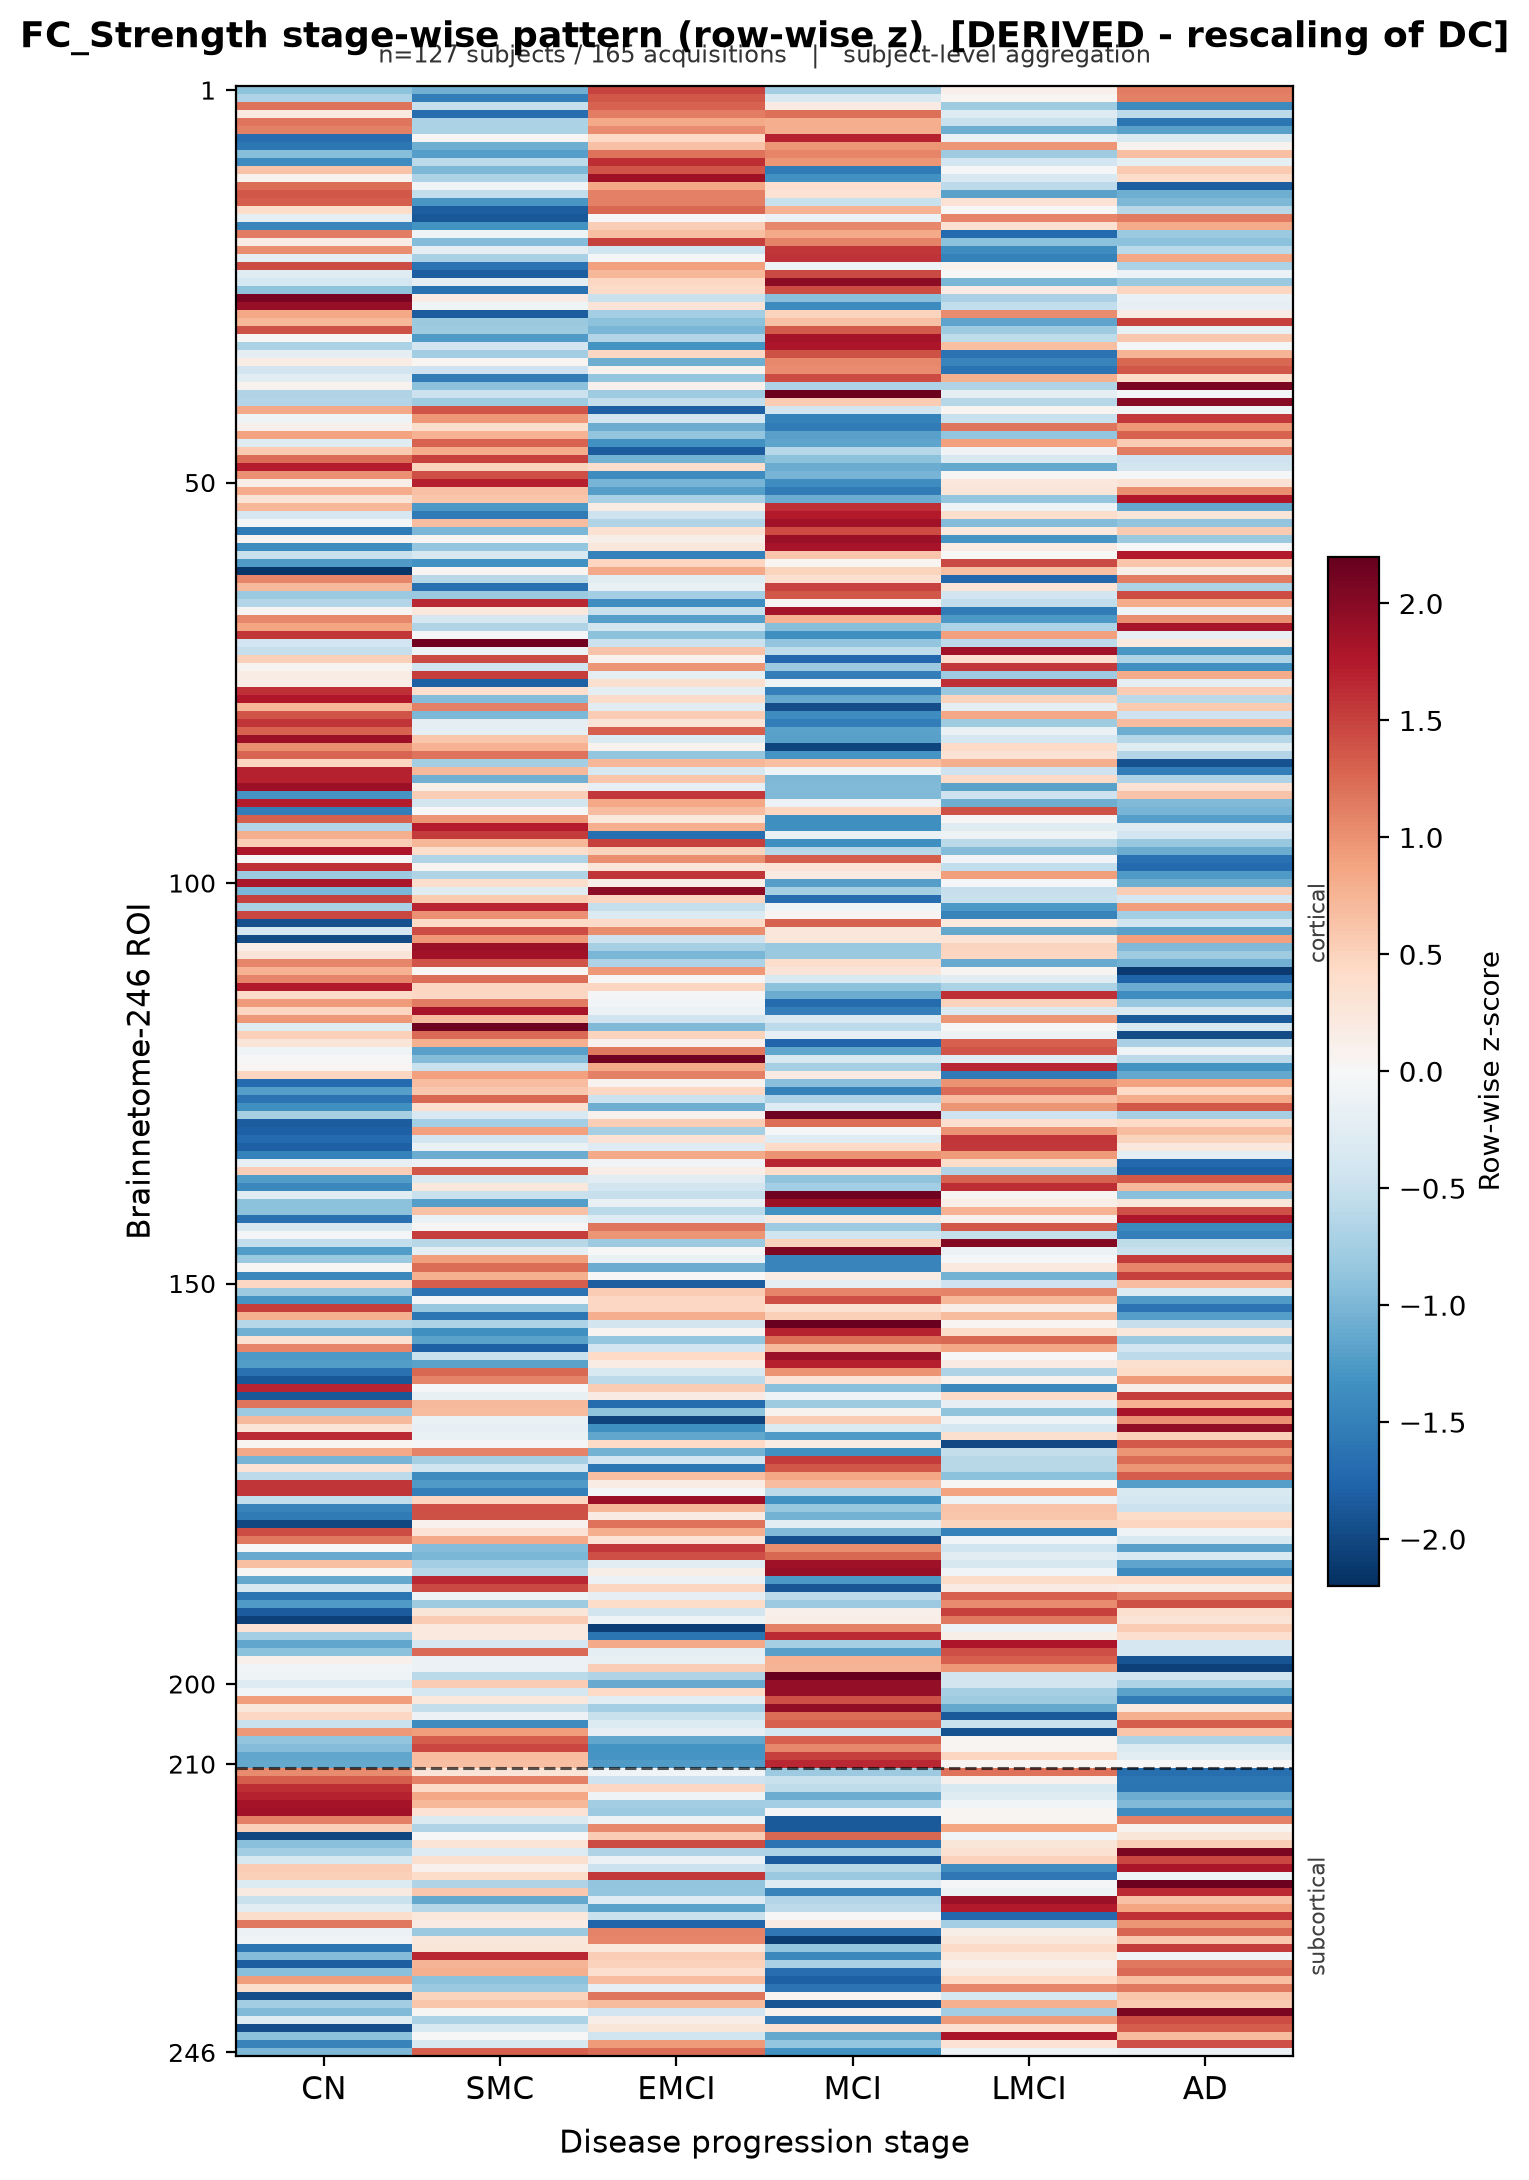
\includegraphics[height=0.44\textheight,keepaspectratio]{figures/FC_Strength_rowz.png}
\caption{DC$_z$ (left) and FC\_Strength (right), rendered independently from
separate stored files. The heatmap panels are identical, because
FC\_Strength $=$ DC$/245$ exactly (maximum difference $6.939\times10^{-18}$ across
all 165 acquisitions, Pearson $r=1.000000000000$); the plotted row-wise $z$ values
differ by at most $6.4\times10^{-15}$. The right-hand file is wider only because its
title carries a ``derived'' tag. FC\_Strength therefore carries no information
independent of DC.}
\label{fig:redundancy}
\end{figure}

\section{Work Not Yet Done}\label{sec:notdone}

To avoid any ambiguity about the scope of this report, the following are \emph{not}
done.
\begin{itemize}
  \item \textbf{Comorbidity data are not cleaned.} Five of the six cohort table
        archives are present; the LMCI tables are missing entirely, leaving 20
        subjects without CDR, MMSE, GDS, medical-history or APOE4 data. Of the 21
        subjects lacking APOE4, 20 are the whole LMCI group, so the missingness is
        group-structured, and an availability indicator would act as a proxy label for
        LMCI. It must not be used as a feature.
  \item \textbf{Hypertension and diabetes are not directly available.} The ADNI
        medical-history tables supply only the broad categories MH4CARD
        (cardiovascular) and MH9ENDO (endocrine); they are used under those names.
  \item \textbf{Modules 4--6 are not started:} the multi-attention transformer,
        meta-learning, comorbidity fusion, the Bayesian ordinal classifier and the
        dashboard. No accuracy, AUC or other performance figure exists, and none is
        implied anywhere in this report.
  \item \textbf{Cross-validation is not built.} Subject-level folds and train-fold-only
        cross-subject scaling are still to be implemented.
\end{itemize}

\section{Discussion}

\textbf{Comparison with conventional practice.} The pipeline departs from a textbook
rs-fMRI workflow at two points, in both cases because the data compels it. A
conventional pipeline co-registers BOLD to a subject T1w image and normalises
through it, and derives tissue regressors from that subject's own segmentation.
Neither is possible here, so EPI-to-template registration is performed directly and
tissue regressors are taken from population priors. This is a genuine limitation
rather than a simplification: direct EPI registration is less precise because EPI
has lower anatomical contrast, and its quality cannot be benchmarked against a
T1w-mediated alternative using this dataset. Equally, a conventional pipeline applies
slice-timing correction; the exhaustive audit described in Chapter~\ref{ch:impl}
establishes this is not available, and the honest response was to omit the step and
document it rather than assume an acquisition order.

\textbf{On scale and feature redundancy.} Two findings will shape the modelling
stage more than any preprocessing choice. First, raw ALFF varies by more than two
orders of magnitude across acquisitions, because it is expressed in units
proportional to raw BOLD intensity, whereas ReHo --- being bounded --- varies only
narrowly. Supplying both unnormalised to a model would allow scanner and protocol
scaling to dominate any biological signal; the within-subject normalisation of
Module~5 addresses this. Second, one of the four nominal biomarkers was found to be
an exact rescaling of another, so the independent regional feature count is three,
not four. Both findings were identified by inspecting the data rather than inherited
from the design, which illustrates the value of auditing features before modelling.

\textbf{Limitations.} Beyond the absence of T1w and slice-timing data, three
limitations bear on the conclusions that can eventually be drawn. The effective
sample is 127 subjects across six ordered classes with a smallest class of 14,
which bounds model capacity and makes a single held-out test split uninformative;
repeated subject-grouped cross-validation is required. Eight acquisitions are
permanently excluded on account of the 6.02\,s TR subgroup unless the filter
specification is revisited for them. Finally, the comorbidity data are incomplete and the gap is group-structured; see
Section~\ref{sec:notdone}, which also records what has not yet been done.

\textbf{Next steps.} Immediate work is to complete the comorbidity table, construct
the subject-level cohort index with fixed stratified grouped cross-validation folds
so that cross-subject scaling can be fitted on training data only, and then
implement the multi-attention transformer and meta-learning blocks. The ordinal
scale used by the classifier is the one fixed at Review~I, namely
CN $\rightarrow$ SMC $\rightarrow$ EMCI $\rightarrow$ MCI $\rightarrow$ LMCI
$\rightarrow$ AD, which orders the three mild-cognitive-impairment cohorts as
early, intermediate and late. This ordering determines the loss structure of the
ordinal model and is therefore held fixed throughout.

\begin{thebibliography}{99}
\bibitem{adnimri} C. R. Jack Jr., M. A. Bernstein, N. C. Fox, et al., ``The
Alzheimer's Disease Neuroimaging Initiative (ADNI): MRI methods,'' \textit{Journal
of Magnetic Resonance Imaging}, vol.~27, no.~4, pp.~685--691, 2008.

\bibitem{adniclinical} R. C. Petersen, P. S. Aisen, L. A. Beckett, et al.,
``Alzheimer's Disease Neuroimaging Initiative (ADNI): clinical characterization,''
\textit{Neurology}, vol.~74, no.~3, pp.~201--209, 2010.

\bibitem{brainnetome} L. Fan, H. Li, J. Zhuo, et al., ``The Human Brainnetome Atlas:
A New Brain Atlas Based on Connectional Architecture,'' \textit{Cerebral Cortex},
vol.~26, no.~8, pp.~3508--3526, 2016.

\bibitem{reho} Y. Zang, T. Jiang, Y. Lu, Y. He, and L. Tian, ``Regional homogeneity
approach to fMRI data analysis,'' \textit{NeuroImage}, vol.~22, no.~1, pp.~394--400,
2004.

\bibitem{alff} Y.-F. Zang, Y. He, C.-Z. Zhu, et al., ``Altered baseline brain
activity in children with ADHD revealed by resting-state functional MRI,''
\textit{Brain and Development}, vol.~29, no.~2, pp.~83--91, 2007.

\bibitem{falff} Q.-H. Zou, C.-Z. Zhu, Y. Yang, et al., ``An improved approach to
detection of amplitude of low-frequency fluctuation (ALFF) for resting-state fMRI:
fractional ALFF,'' \textit{Journal of Neuroscience Methods}, vol.~172, no.~1,
pp.~137--141, 2008.

\bibitem{centrality} X.-N. Zuo, R. Ehmke, M. Mennes, et al., ``Network centrality in
the human functional connectome,'' \textit{Cerebral Cortex}, vol.~22, no.~8,
pp.~1862--1875, 2012.

\bibitem{fd} J. D. Power, K. A. Barnes, A. Z. Snyder, B. L. Schlaggar, and S. E.
Petersen, ``Spurious but systematic correlations in functional connectivity MRI
networks arise from subject motion,'' \textit{NeuroImage}, vol.~59, no.~3,
pp.~2142--2154, 2012.

\bibitem{friston24} K. J. Friston, S. Williams, R. Howard, R. S. J. Frackowiak, and
R. Turner, ``Movement-related effects in fMRI time-series,'' \textit{Magnetic
Resonance in Medicine}, vol.~35, no.~3, pp.~346--355, 1996.

\bibitem{ants} B. B. Avants, C. L. Epstein, M. Grossman, and J. C. Gee, ``Symmetric
diffeomorphic image registration with cross-correlation: evaluating automated
labeling of elderly and neurodegenerative brain,'' \textit{Medical Image Analysis},
vol.~12, no.~1, pp.~26--41, 2008.

\bibitem{freesurfer} B. Fischl, ``FreeSurfer,'' \textit{NeuroImage}, vol.~62, no.~2,
pp.~774--781, 2012.

\bibitem{afni} R. W. Cox, ``AFNI: software for analysis and visualization of
functional magnetic resonance neuroimages,'' \textit{Computers and Biomedical
Research}, vol.~29, no.~3, pp.~162--173, 1996.
\end{thebibliography}

\end{document}
